%1644
\newpage

\section{ジャンプアクションゲームに挑戦しよう}


\subsection{ジャンプアクションゲームのあそびかた}



ジャンプアップゲームでキャラクターを動かして遊ぶ\ruby{本格的}{ほん|かく|てき}なゲームを\ruby{体験}{たい|けん}してみましょう。


ファイル→「開く」メニューから「jump.hsp」を読み込んでください。

見つからない場合は、まわりの友達か、近くの先生に聞いてみてください。

[F5]キーで実行すると、タイトル画面が出ます。[Enter]キーを押して始めてください。


\begin{figure}[H]
    \begin{center}
      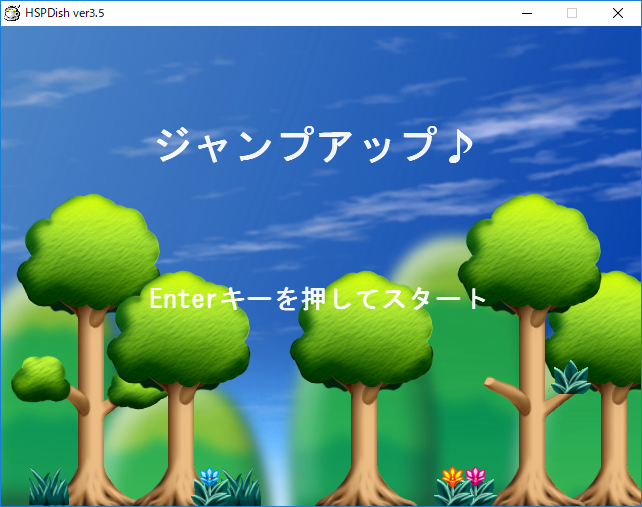
\includegraphics[keepaspectratio,width=11.192cm,height=8.827cm]{text04-img/s_jumptitle.png}
      \caption{タイトル画面}
    \end{center}
    \label{fig:prog_menu}
\end{figure}

ジャンプアップゲームは、キャラクターを操作してコインを取るゲームです。

左右の移動とジャンプをさせることができます。



\begin{figure}[H]
    \begin{center}
      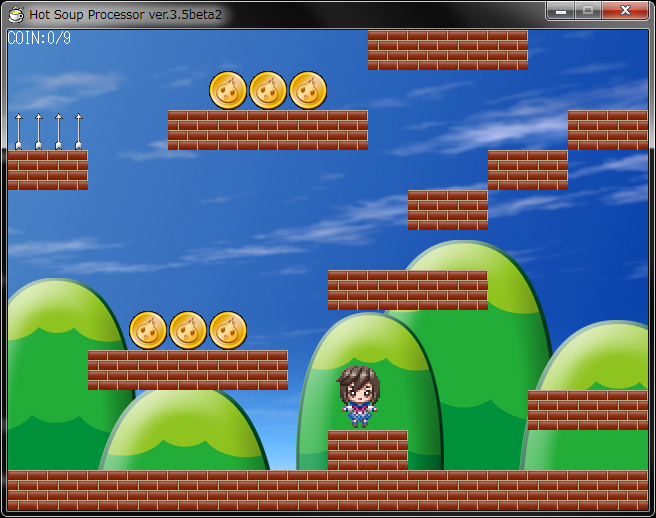
\includegraphics[keepaspectratio,width=11.28cm,height=8.915cm]{text04-img/s_jumpgame.png}
      \caption{ジャンプアップゲーム画面}
    \end{center}
    \label{fig:prog_menu}
\end{figure}

\ruby{矢印}{や|じるし}のキーで左右に動かして、スペースキーでジャンプです。

ジャンプしながら、コインを取って上に進みましょう。

すべてのコインを取るとあなたの勝ちです。逆に、\ruby{地面}{じ|めん}に置かれている\ruby{矢}{や}に当たってしまうとゲームオーバーになってしまいます。


\begin{figure}[H]
    \begin{center}
      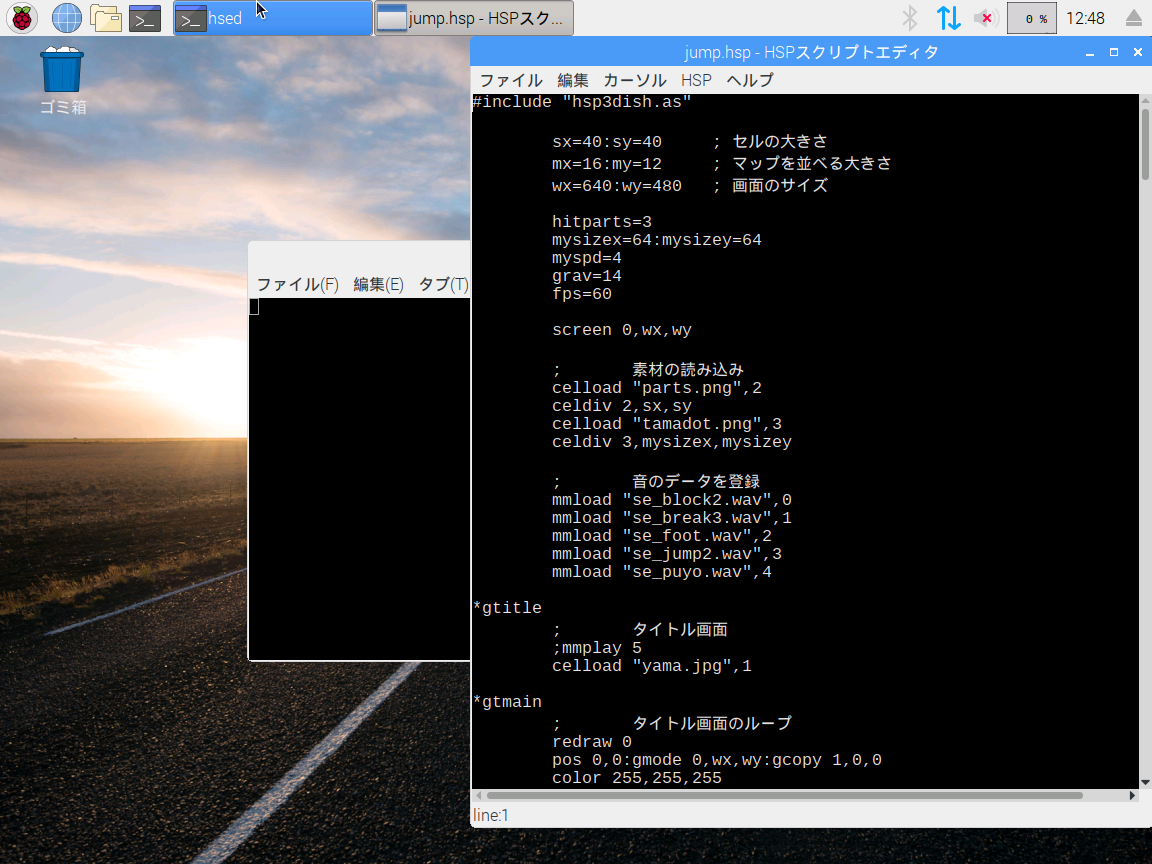
\includegraphics[keepaspectratio,width=11.192cm,height=8.393cm]{text04-img/s_jumpsrc.png}
      \caption{ジャンプアップゲームのプログラム}
    \end{center}
    \label{fig:prog_menu}
\end{figure}

\newpage
\subsection{例題に挑戦しよう}

ゲームが遊べた人は、以下の例題にも挑戦してみよう。

・オリジナルの面を作ってみよう

・ゲームの動きを改造してみよう

・ゲームの背景や絵を改造してみよう

・ゲームのタイトル画面を改造してみよう

例題の考え方がわからない時は、近くのTAか先生に聞いてください。

わからない所は、そのままにせず、必ず答えを見つけてから先に進みましょう。

%1747
%1747
\newpage
\subsection{例題4-8 オリジナルの面を作ってみよう}


\begin{description}
    \item \textgt{\bf  考え方}
\end{description}

ジャンプアップゲーム(jump.hsp)のプログラムを改造してゲームで使われている\ruby{面}{めん}(マップ)を変えてみましょう。

プログラムを編集することで、面のデータを自分で変えることができます。

以下の場所を探して修正します。


\begin{figure}[H]
    \begin{center}
      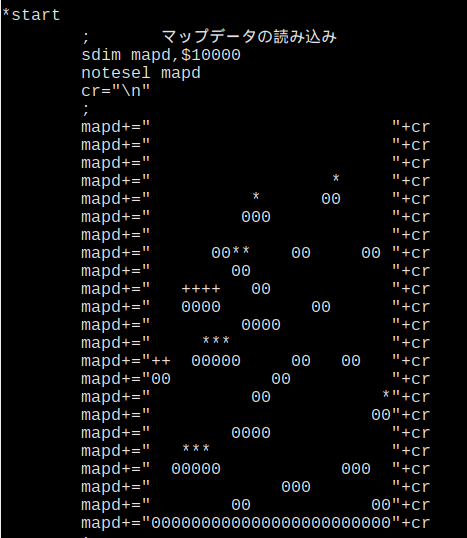
\includegraphics[keepaspectratio,width=10.478cm,height=12.07cm]{text04-img/s_jumpmapsrc.png}
    \end{center}
    \label{fig:prog_menu}
\end{figure}



\begin{description}
    \item \textgt{\bf \ \ 「0」はレンガ(壁)になります。}
    \item \textgt{\bf \ \ 「*」はコイン、「+」は矢になります。}
    \item \textgt{\bf \ \ マップデータが書かれている場所を探して、自分だけの面を作ってみましょう。}
\end{description}

でたらめに書き直してもエラーが出るだけです。必ず、

\begin{description}
    \item \textgt{\bf \ \ mapd+=” \ \ \ \ \ \ \ \ \ \ \ \ \ \ \ \ \ \ \ \ \ \ \ \ \ \ \ \ “+cr}
\end{description}

という形になるようにしてください。

文字は「”」で囲み、最後に「+cr」を入れます。

面のデータは、縦・横方向に広げることができます。


\begin{description}
    \item \textgt{\bf 例題4-8 答え}
\end{description}

ゲームを改造することで、難しくなったり、簡単になったりします。

改造ができたらTAや周りの友達にも見せてあげましょう。

%1820
%1820
\newpage
\subsection{例題4-9 ゲームの動きを改造してみよう}

\begin{description}
    \item \textgt{\bf  考え方}
\end{description}



ジャンプアップゲーム(jump.hsp)のプログラムは、ゲームの動きを決める変数に決められた値が代入されています。

\ruby{慣}{な}れてきたら、改造できる部分を自分で探してみましょう。



\begin{figure}[H]
    \begin{center}
      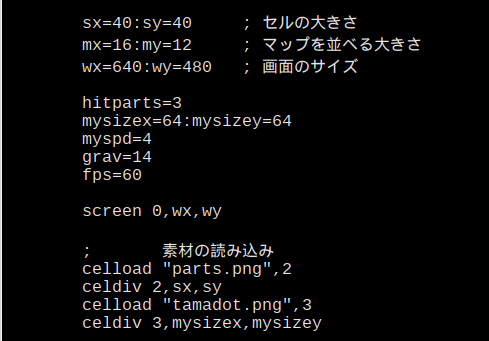
\includegraphics[keepaspectratio,width=11.853cm,height=8.266cm]{text04-img/s_jumpsrcpart.png}
    \end{center}
    \label{fig:prog_menu}
\end{figure}


「セルの大きさ」「マップを並べる大きさ」「画面のサイズ」はそのままにしておいてください。

mypd、gravといった変数の値を変えるとどうなるか、試してみましょう。

\begin{description}
    \item \textgt{\bf  例題4-9 答え}
\end{description}

「myspd=4」が歩くスピードを決めています

「grav=14」がジャンプの強さを決めています

動きが変わったら、どんな値だと良いバランスのゲームになるか考えてみましょう。

改造ができたらTAや周りの友達にも見せてあげましょう。


%1881
%1881
\newpage
\subsection{例題4-10 ゲームの背景や絵を改造してみよう}


\begin{description}
    \item \textgt{\bf  考え方}
\end{description}

ジャンプアップゲーム(jump.hsp)のプログラムで使われている画像を確認してみましょう。

画像を書き換えて、自分だけのゲーム画面を作ることもできます。

\begin{figure}[H]
    \begin{center}
      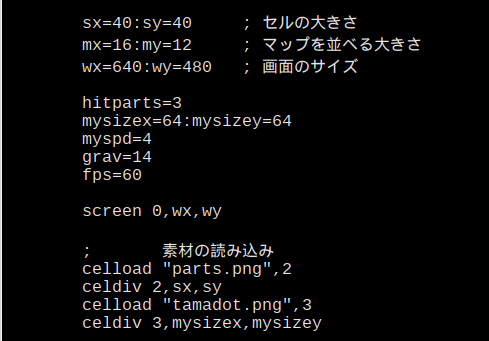
\includegraphics[keepaspectratio]{text04-img/s_jumpsrcpart.png}
    \end{center}
    \label{fig:prog_menu}
\end{figure}

celload命令で読み込まれているファイルが、ゲームに出てくる画像となります。

操作する主人公は「tamadot.png」という画像です

面を構成するパーツは、「parts.png」という画像にまとめられています。

\begin{figure}[H]
    \begin{center}
      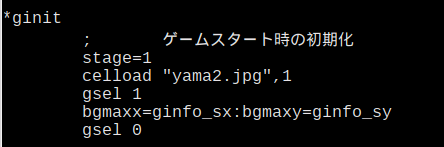
\includegraphics[keepaspectratio,width=10.689cm,height=3.538cm]{text04-img/s_jumpbackgroundsrc.png}
    \end{center}
    \label{fig:prog_menu}
\end{figure}

また、ゲームの背景は、「yama2.jpg」という画像が使われています。

それぞれが、どんな役割を果たしているか、GIMPなどのツールで確認してみましょう。



\begin{description}
    \item \textgt{\bf 例題4-10 答え}
\end{description}



ジャンプアップゲームの背景は、実は小さな絵を並べて、大きな世界を作っています。

GIMPを使って、ジャンプアップゲームの絵を改造してみましょう。

小さな絵を実際に見て改造をしてみましょう。以前にやった手順を覚えていますか?

「parts.png」アイコンの右クリックメニューから「GNU Image Manipulation Program」をクリックして、GIMPツールを起動させましょう。


\begin{figure}[H]
    \begin{center}
      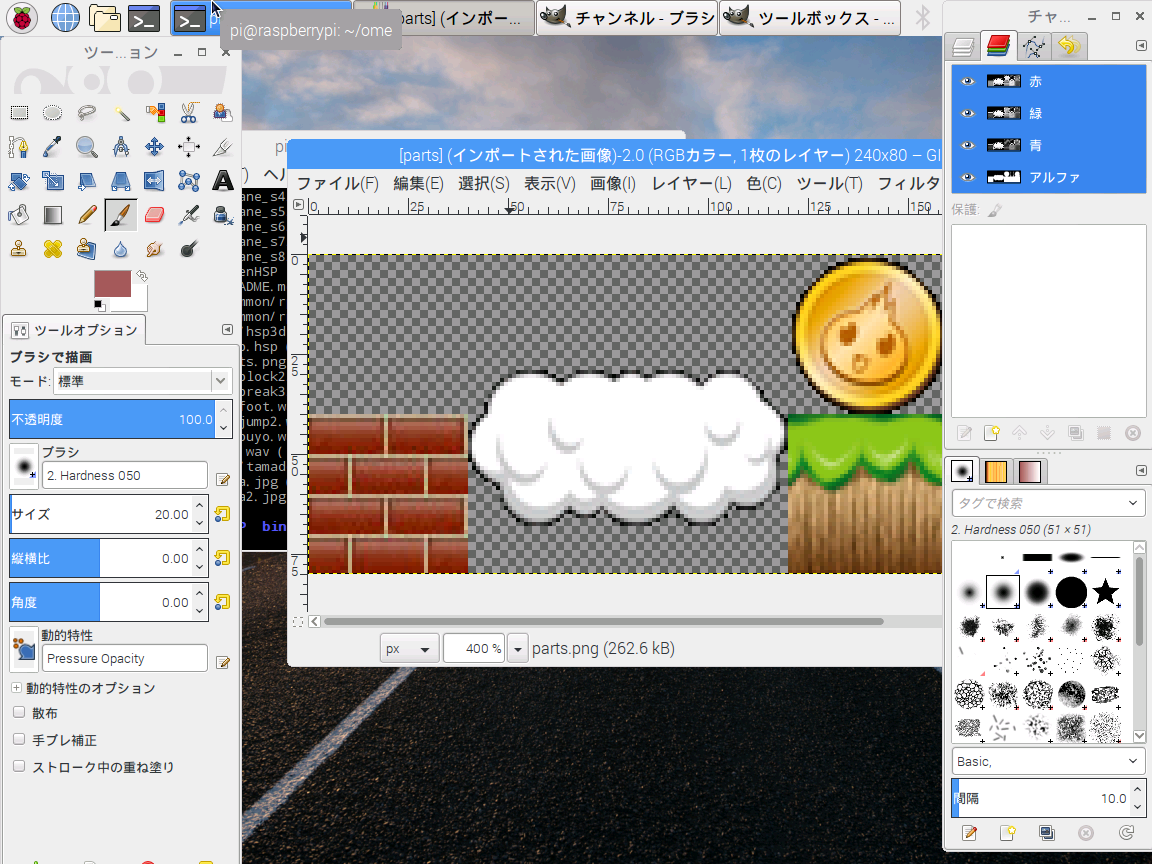
\includegraphics[keepaspectratio,width=12.065cm,height=9.049cm]{text04-img/s_gimpeditjumppart.png}
      \caption{parts.pngを修正している画面}
    \end{center}
    \label{fig:prog_menu}
\end{figure}

パレットで色を選んで、\ruby{鉛筆}{えん|ぴつ}のツールで絵を書いていきます。


\begin{figure}[H]
    \begin{center}
      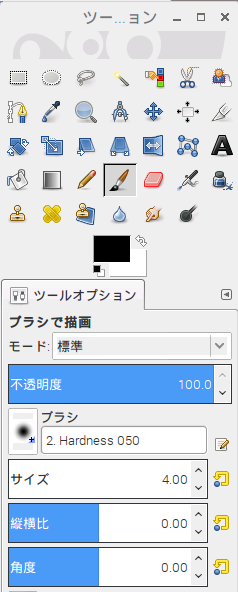
\includegraphics[keepaspectratio,width=4.075cm,height=10.16cm]{text04-img/s_gimppalette.png}
    \end{center}
    \label{fig:prog_menu}
\end{figure}


元の絵があった部分を書き換えて他の\ruby{絵柄}{え|がら}にしてみましょう。

画像が小さい場合は、画像の下にある「100\%」の右側にあるボタンを押して、「400\%」「800\%」などを選ぶと拡大されます。

絵を修正する時には、ツールアイコンの中から「ブラシ」を選択して、サイズを4〜6くらいの数字に変えてから絵の上で、マウスボタンを押しながら動かして色を置きます。


色を変更する場合は、ツールパレットの描画色をクリックして、「描画色の変更」ダイアログを出してから好きな色を選びます。

\begin{figure}[H]
    \begin{center}
      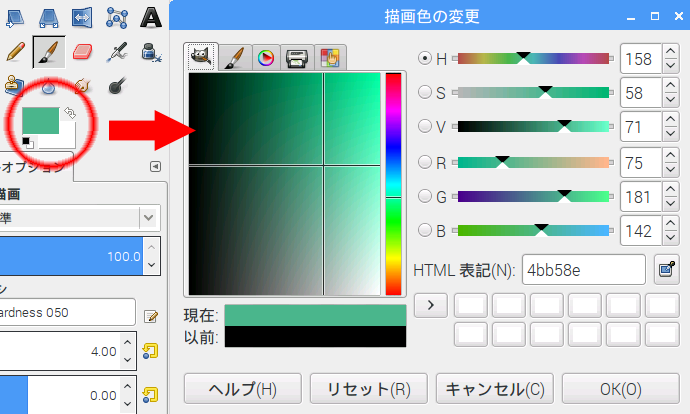
\includegraphics[keepaspectratio,width=10.993cm,height=6.588cm]{text04-img/s_gimpchangecolor.png}
    \end{center}
    \label{fig:prog_menu}
\end{figure}

元の絵を書き換えたら、ファイル→「parts.pngに上書きエクスポート」を選んで保存します。
\clearpage


背景画像は、縦長のもので「yama2.jpg」として保存されています。変更した画像でゲームを動かしてみましょう。

[F5]キーを押して実行して変わっていれば成功です。

改造ができたらTAや周りの友達にも見せてあげましょう。


\begin{figure}[H]
    \begin{center}
      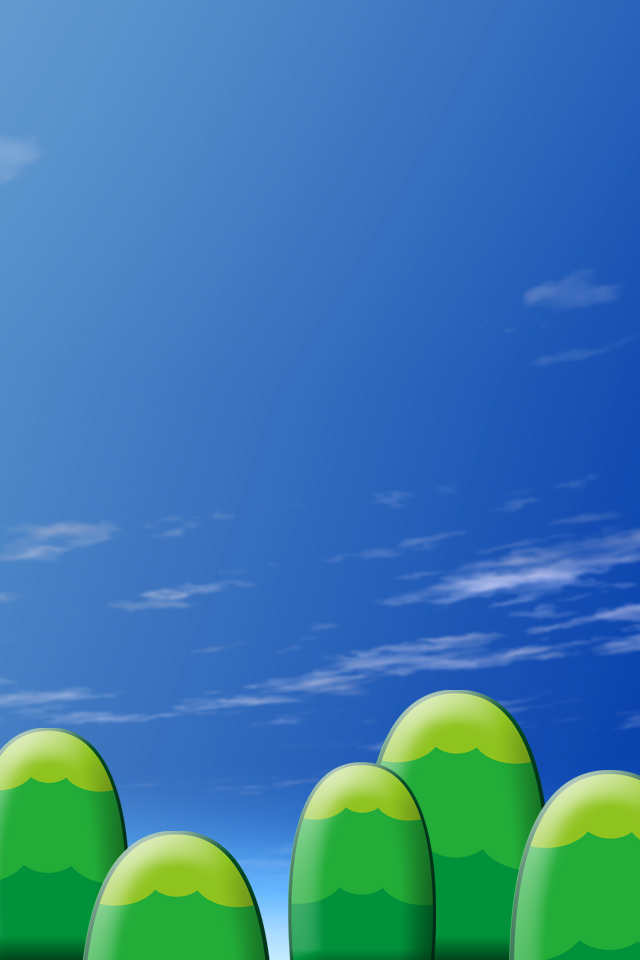
\includegraphics[keepaspectratio,width=8.546cm,height=12.804cm]{text04-img/s_yama2.jpg}
      \caption{画像ファイル yama2.jpgの内容}
    \end{center}
    \label{fig:prog_menu}
\end{figure}

%2038
%2038
\newpage
\subsection{例題4-11 ゲームのタイトル画面を改造してみよう}


\begin{description}
    \item \textgt{\bf  考え方}
\end{description}


ジャンプアップゲーム(jump.hsp)のプログラムを改造して、タイトル画面を自分だけのものにしてみましょう。

\begin{figure}[H]
    \begin{center}
      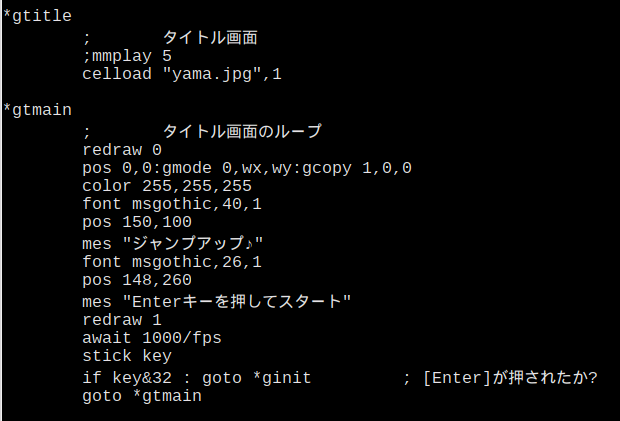
\includegraphics[keepaspectratio,width=14.42cm,height=9.791cm]{text04-img/s_jumptitlesrc.png}
    \end{center}
    \label{fig:prog_menu}
\end{figure}


\begin{description}
    \item \textgt{\bf  例題4-11 答え}
\end{description}

背景の画像に「yama.jpg」、後は決められたサイズと色で文字を出しています。

「ジャンプアップ」ではない、別なタイトルを考えてみましょう。

どんな画面にしたいか、考えてから改造を始めましょう。

改造ができたらTAや周りの友達にも見せてあげましょう。



% Last Part:

%2083